\subsection{Devices Configuration}

\subsubsection*{R5}
The Router5 is a clone of the Router1.
The network of this router is composed by two enabled adapters:
\begin{itemize}
	\item Adapter 1: Internal Network (Name: intnet);
	\item Adapter 2: NAT Network (Name: NatNetwork).
\end{itemize}
After the start of the machine it is setted with this commands:

\lstinputlisting[language=bash]{cfg_files/r5.txt}

\subsection*{R1}
\lstinputlisting[language=bash]{cfg_files/r1.txt}

\subsection*{Kali-PC1}
\lstinputlisting[language=bash]{cfg_files/Kali-PC1_interfaces}

\subsection*{Kali-PC1}
\lstinputlisting[language=bash]{cfg_files/Kali-PC2_interfaces}

\subsection*{XP1}
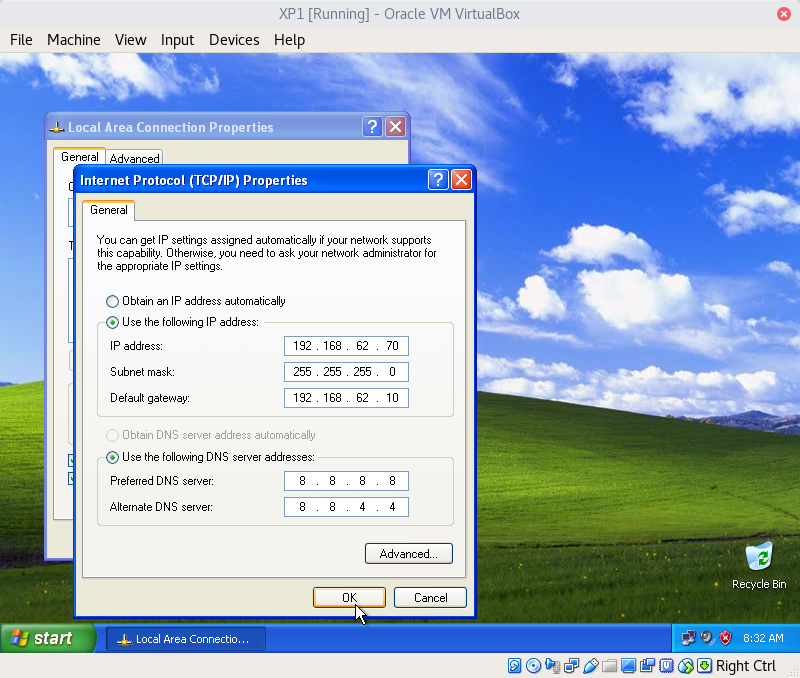
\includegraphics[height=7cm]{img/WinXPNetworkConfiguration}\par
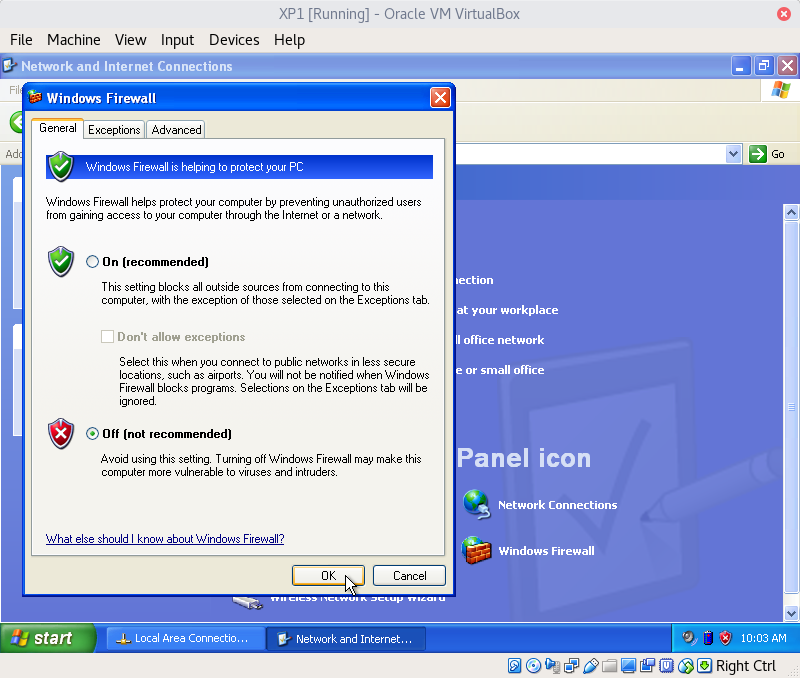
\includegraphics[height=7cm]{img/WinXPFirewallDisabled}\par